%%%%%%%%%%%%%%%%%%%%%%%%%%%%%%%%%%%%%%%%%%%%%%%%%%%
%% LaTeX book template                           %%
%% Author:  Amber Jain (http://amberj.devio.us/) %%
%% License: ISC license                          %%
%%%%%%%%%%%%%%%%%%%%%%%%%%%%%%%%%%%%%%%%%%%%%%%%%%%

\documentclass[a4paper,11pt,oneside]{book}
\usepackage{../../modulestyle}

%%%%%%%%%%%%%%%%%%%%%%%%%%%%%%%%%%%%%%%%%%%%%%%%%%%%%%%%%
% Source: http://en.wikibooks.org/wiki/LaTeX/Hyperlinks %
%%%%%%%%%%%%%%%%%%%%%%%%%%%%%%%%%%%%%%%%%%%%%%%%%%%%%%%%%

%%%%%%%%%%%%%%%%%%%%%%%%%%%%%%%%%%%%%%%%%%%%%%%%%%%%%%%%%%%%%%%%%%%%%%%%%%%%%%%%
% 'dedication' environment: To add a dedication paragraph at the start of book %
% Source: http://www.tug.org/pipermail/texhax/2010-June/015184.html            %
%%%%%%%%%%%%%%%%%%%%%%%%%%%%%%%%%%%%%%%%%%%%%%%%%%%%%%%%%%%%%%%%%%%%%%%%%%%%%%%%
\newenvironment{dedication}
{
   \cleardoublepage
   \thispagestyle{empty}
   \vspace*{\stretch{1}}
   \hfill\begin{minipage}[t]{0.66\textwidth}
   \raggedright
}
{
   \end{minipage}
   \vspace*{\stretch{3}}
   \clearpage
}

%%%%%%%%%%%%%%%%%%%%%%%%%%%%%%%%%%%%%%%%%%%%%%%%
% Chapter quote at the start of chapter        %
% Source: http://tex.stackexchange.com/a/53380 %
%%%%%%%%%%%%%%%%%%%%%%%%%%%%%%%%%%%%%%%%%%%%%%%%
\makeatletter
\renewcommand{\@chapapp}{}% Not necessary...
\newenvironment{chapquote}[2][2em]
  {\setlength{\@tempdima}{#1}%
   \def\chapquote@author{#2}%
   \parshape 1 \@tempdima \dimexpr\textwidth-2\@tempdima\relax%
   \itshape}
  {\par\normalfont\hfill--\ \chapquote@author\hspace*{\@tempdima}\par\bigskip}
\makeatother

%%%%%%%%%%%%%%%%%%%%%%%%%%%%%%%%%%%%%%%%%%%%%%%%%%%
% First page of book which contains 'stuff' like: %
%  - Book title, subtitle                         %
%  - Book author name                             %
%%%%%%%%%%%%%%%%%%%%%%%%%%%%%%%%%%%%%%%%%%%%%%%%%%%

\newcommand{\CourseTitle}{Data Structures and Algorithms}
\newcommand{\ChapterNumber}{2}
\newcommand{\ChapterTitle}{Arrays and Linked Lists}
\newcommand{\CodingNumber}{2}

% A Catchy Title to be displayed on the first page
\newcommand{\CodingTitle}{Going in Circles}
\newcommand{\SubmissionDeadline}{October 18, 2024}
\newcommand{\SubmissionDeadlineText}{on or before \SubmissionDeadline}
\newcommand{\SubmissionTemplateURL}{https://docs.google.com/document/d/1zZf3W0Hj6NfCGU7sKAaz_cztSER5e7Vx/edit?usp=sharing&ouid=112709378145681657270&rtpof=true&sd=true}

\newcommand{\BookTitle}{Coding Exercise: \CodingNumber - \CodingTitle}
\newcommand{\BookTitleFootnote}{A coding exercise for
\textnormal{Chapter \ChapterNumber} of the Study Guide on the course \CourseTitle.}

\newcommand{\BookSubtitle}{Chapter \ChapterNumber: \ChapterTitle}
\newcommand{\BookSubtitleFootnote}{This chapter introduces the concepts of arrays and linked lists.}

\newcommand{\BookAuthorFirstName}{Jarrian Vince}
\newcommand{\BookAuthorLastName}{Gojar}
\newcommand{\BookAuthorName}{Jarrian Vince G. Gojar}
\newcommand{\BookAuthorURL}{https://github.com/godkingjay}

\newcommand{\GoogleDriveURLBSITTwoFour}{https://drive.google.com/drive/folders/1uc3ehhK4Mv84KXPe8oV3l3AGI6czVhBx?usp=sharing}
\newcommand{\GoogleDriveURLBSITTwoFive}{https://drive.google.com/drive/folders/1eIkUp3t2cAKIpd9KZGbQlZEGU516S_sE?usp=sharing}

\newcommand{\FolderFormat}{Group Number - LastName1\_FirstName1, LastName2\_FirstName2}
\newcommand{\FolderFormatExample}{Group 1 - Doe\_John, Smith\_Jane}

% Book's title and subtitle
\title{\Huge \textbf{\BookTitle}  \footnote{\BookTitleFootnote} \\
\huge \BookSubtitle \footnote{\BookSubtitleFootnote}}

% Author
\author{\textsc{\BookAuthorName}\thanks{\url{\BookAuthorURL}}}

\begin{document}

\frontmatter
\date{}
\maketitle

%%%%%%%%%%%%%%%%%%%%%%%%%%%%%%%%%%%%%%%%%%%%%%%%%%%%%%%%%%%%%%%
% Add a dedication paragraph to dedicate your book to someone %
%%%%%%%%%%%%%%%%%%%%%%%%%%%%%%%%%%%%%%%%%%%%%%%%%%%%%%%%%%%%%%%
\begin{dedication}
Sorsogon State University - Bulan Campus
\end{dedication}

%%%%%%%%%%%%%%%%%%%%%%%%%%%%%%%%%%%%%%%%%%%%%%%%%%%%%%%%%%%%%%%%%%%%%%%%
% Auto-generated table of contents, list of figures and list of tables %
%%%%%%%%%%%%%%%%%%%%%%%%%%%%%%%%%%%%%%%%%%%%%%%%%%%%%%%%%%%%%%%%%%%%%%%%

\mainmatter

%%%%%%%%%%%
% Preface %
%%%%%%%%%%%
\section*{Coding Exercises}

\begin{chapquote}{Bjarne Stroustrup}
``C makes it easy to shoot yourself in the foot; C++ makes it harder, but when
you do, it blows away your whole leg.''
\end{chapquote}

Instructions: Write a program that solves the following problems.
Submit your code to the Google Drive folder provided by the instructor.

% The following are the exercises

\begin{enumerate}
  % Reverse an Array
  \item \textbf{Reverse an Array:} Write a C++ program to reverse an array of
  integers. The program should take the size of the array and the elements of
  the array as input and output the reversed array.
  \begin{enumerate}
      \item Declare an array of integers with a fixed size.
      \begin{align*}
          \text{int arr[6];}
      \end{align*}
      \item Initialize the array with the input elements.
      \begin{align*}
          \text{arr = \{19, 10, 8, 17, 9, 15\};}
      \end{align*}
      \item Reverse the array using a loop. \\
      \begin{center}
        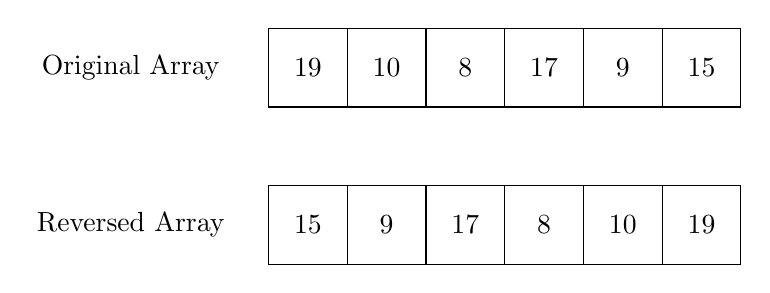
\begin{tikzpicture}[scale=1]
          \draw (0, 0) grid (6, 1);
          \node at (0.5, 0.5) {19};
          \node at (1.5, 0.5) {10};
          \node at (2.5, 0.5) {8};
          \node at (3.5, 0.5) {17};
          \node at (4.5, 0.5) {9};
          \node at (5.5, 0.5) {15};
          \node at (-1.75, 0.5) {Original Array};

          % \draw[->] (3, 0) -- (3, -1);

          \draw (0, -1) grid (6, -2);
          \node at (0.5, -1.5) {15};
          \node at (1.5, -1.5) {9};
          \node at (2.5, -1.5) {17};
          \node at (3.5, -1.5) {8};
          \node at (4.5, -1.5) {10};
          \node at (5.5, -1.5) {19};
          \node at (-1.75, -1.5) {Reversed Array};
        \end{tikzpicture}
      \end{center}
      \item Print the reversed array to the console.
      \begin{align*}
          \text{Reversed Array: 15, 9, 17, 8, 10, 19}
      \end{align*}
      \item Determine the \textbf{time complexity} and
      \textbf{space complexity} of the program.
  \end{enumerate}

  % Reverse a Linked List
  \item \textbf{Reverse a Linked List:} Write a C++ program to reverse a singly
  linked list. The program should take the elements of the linked list as input
  and output the reversed linked list.

  \begin{enumerate}
      \item Create a singly linked list with nodes containing the elements
      \begin{center}
          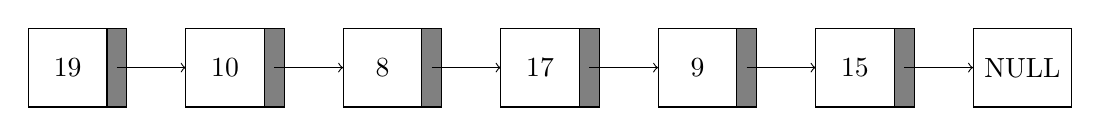
\begin{tikzpicture}
              \draw (0, 0) rectangle (1, 1);
              \node at (0.5, 0.5) {19};
              \draw[fill=gray] (1, 1) rectangle (1.25, 0);
  
              \draw (2, 0) rectangle (3, 1);
              \node at (2.5, 0.5) {10};
              \draw[fill=gray] (3, 1) rectangle (3.25, 0);
  
              \draw (4, 0) rectangle (5, 1);
              \node at (4.5, 0.5) {8};
              \draw[fill=gray] (5, 1) rectangle (5.25, 0);
  
              \draw (6, 0) rectangle (7, 1);
              \node at (6.5, 0.5) {17};
              \draw[fill=gray] (7, 1) rectangle (7.25, 0);
  
              \draw (8, 0) rectangle (9, 1);
              \node at (8.5, 0.5) {9};
              \draw[fill=gray] (9, 1) rectangle (9.25, 0);
  
              \draw (10, 0) rectangle (11, 1);
              \node at (10.5, 0.5) {15};
              \draw[fill=gray] (11, 1) rectangle (11.25, 0);
  
              \draw (12, 0) rectangle (13.25, 1);
              \node at (12.625, 0.5) {NULL};
  
              \draw[->] (1.125, 0.5) -- (2, 0.5);
              \draw[->] (3.125, 0.5) -- (4, 0.5);
              \draw[->] (5.125, 0.5) -- (6, 0.5);
              \draw[->] (7.125, 0.5) -- (8, 0.5);
              \draw[->] (9.125, 0.5) -- (10, 0.5);
              \draw[->] (11.125, 0.5) -- (12, 0.5);
          \end{tikzpicture}
      \end{center}
      \item Reverse the linked list using a loop.
      \begin{center}
          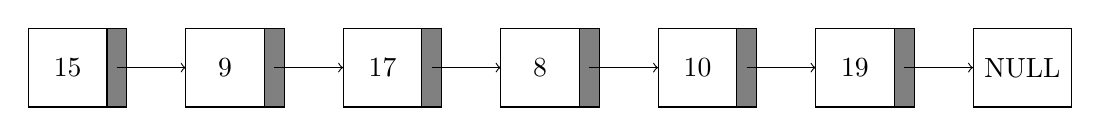
\begin{tikzpicture}
              \draw (0, 0) rectangle (1, 1);
              \node at (0.5, 0.5) {15};
              \draw[fill=gray] (1, 1) rectangle (1.25, 0);
  
              \draw (2, 0) rectangle (3, 1);
              \node at (2.5, 0.5) {9};
              \draw[fill=gray] (3, 1) rectangle (3.25, 0);
  
              \draw (4, 0) rectangle (5, 1);
              \node at (4.5, 0.5) {17};
              \draw[fill=gray] (5, 1) rectangle (5.25, 0);
  
              \draw (6, 0) rectangle (7, 1);
              \node at (6.5, 0.5) {8};
              \draw[fill=gray] (7, 1) rectangle (7.25, 0);
  
              \draw (8, 0) rectangle (9, 1);
              \node at (8.5, 0.5) {10};
              \draw[fill=gray] (9, 1) rectangle (9.25, 0);
  
              \draw (10, 0) rectangle (11, 1);
              \node at (10.5, 0.5) {19};
              \draw[fill=gray] (11, 1) rectangle (11.25, 0);
  
              \draw (12, 0) rectangle (13.25, 1);
              \node at (12.625, 0.5) {NULL};
  
              \draw[->] (1.125, 0.5) -- (2, 0.5);
              \draw[->] (3.125, 0.5) -- (4, 0.5);
              \draw[->] (5.125, 0.5) -- (6, 0.5);
              \draw[->] (7.125, 0.5) -- (8, 0.5);
              \draw[->] (9.125, 0.5) -- (10, 0.5);
              \draw[->] (11.125, 0.5) -- (12, 0.5);
          \end{tikzpicture}
      \end{center}
      \item Print the reversed linked list to the console.
      \begin{align*}
          \text{Reversed Linked List: 15, 9, 17, 8, 10, 19}
      \end{align*}
      \item Determine the \textbf{time complexity} and
      \textbf{space complexity} of the program.
  \end{enumerate}
  
  % Search a Circular Linked List
  \item \textbf{Search a Circular Linked List:} Write a C++ program to search
  for an element in a circular linked list. The program should take the elements
  of the circular linked list as input and output the position of the element
  in the list. If the current node's next pointer points to the head node, the
  list is circular. If the element is not found in the list, output "Element not
  found." Else, output the position of the element in the list.
  \begin{enumerate}
      \item \textnormal{Create a circular linked list with nodes containing the elements}
      \begin{center}
        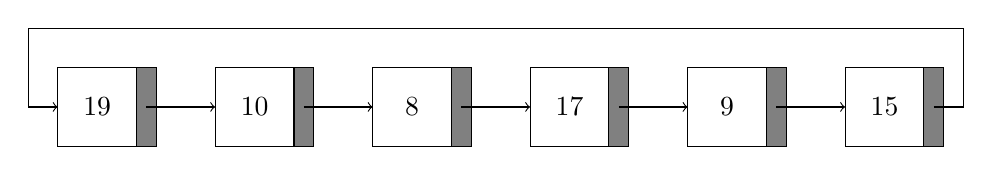
\begin{tikzpicture}
          % Draw the nodes of the circular linked list
          \draw (0, 0) rectangle (1, 1);
          \node at (0.5, 0.5) {19};
          \draw[fill=gray] (1, 1) rectangle (1.25, 0);
  
          \draw (2, 0) rectangle (3, 1);
          \node at (2.5, 0.5) {10};
          \draw[fill=gray] (3, 1) rectangle (3.25, 0);
  
          \draw (4, 0) rectangle (5, 1);
          \node at (4.5, 0.5) {8};
          \draw[fill=gray] (5, 1) rectangle (5.25, 0);
  
          \draw (6, 0) rectangle (7, 1);
          \node at (6.5, 0.5) {17};
          \draw[fill=gray] (7, 1) rectangle (7.25, 0);
  
          \draw (8, 0) rectangle (9, 1);
          \node at (8.5, 0.5) {9};
          \draw[fill=gray] (9, 1) rectangle (9.25, 0);
  
          \draw (10, 0) rectangle (11, 1);
          \node at (10.5, 0.5) {15};
          \draw[fill=gray] (11, 1) rectangle (11.25, 0);
  
          % Draw the arrows between the nodes
          \draw[->] (1.125, 0.5) -- (2, 0.5);
          \draw[->] (3.125, 0.5) -- (4, 0.5);
          \draw[->] (5.125, 0.5) -- (6, 0.5);
          \draw[->] (7.125, 0.5) -- (8, 0.5);
          \draw[->] (9.125, 0.5) -- (10, 0.5);
  
          % Add A Cornered Arrow
          % \draw[->] (11.125, 0.5) to [out=45, in=135] (0, 0.5);
          \draw[->] (11.125, 0.5)
                -- (11.5, 0.5)
                -- (11.5, 1.5)
                -- (-0.375, 1.5)
                -- (-0.375, 0.5)
                -- (0, 0.5);
        \end{tikzpicture}
      \end{center}
      
      \item Using \textit{cin}, take the input element to search for
      \begin{align*}
          \text{Search Element: 21}
      \end{align*}
      \item Search for the element in the circular linked list
      \begin{align*}
          \text{Output: Element not found.}
      \end{align*}
      \item Determine the \textbf{time complexity} and
      \textbf{space complexity} of the program.
  \end{enumerate}
\end{enumerate}

\section*{Submission of Coding Exercises}

Instructions:
\begin{enumerate}
  \item Go to the Google Drive folder provided by the instructor: \\
  \begin{quote}
    \textbf{BSIT 2-4:} \\ \url{\GoogleDriveURLBSITTwoFour} \\ \\
    \textbf{BSIT 2-5:} \\ \url{\GoogleDriveURLBSITTwoFive}
  \end{quote}
  \item Inside the folder, create another folder for your group
  with the following format:
    \begin{quote}
      \textbf{\FolderFormat} \\
      Example: \textbf{\FolderFormatExample}
    \end{quote}
  \item Inside the sub-folder, create another folder with the name:
    \begin{quote}
        \textbf{Chapter \ChapterNumber - Coding Exercise \CodingNumber - \CodingTitle}
    \end{quote}
  \item Inside the folder, upload the file of your submission.
    \begin{quote}
        Fill in the template provided in the following link and upload
        it inside the folder: \\
        \url{\SubmissionTemplateURL}
    \end{quote}
  \item The activity must be submitted \textbf{\SubmissionDeadlineText}.
  \item Late submissions will not be accepted.
\end{enumerate}

\end{document}